\section{Obtaining and building the PCIe Engine}
The repository is divided in several directories:
\begin{table}[H]
	\centering
	\begin{tabularx}{\textwidth}{|l|X|}
	\hline
	\textbf{directory}&\textbf{contents}\\
	\hline
	firmware/constraints&Contains an XDC file with Vivado constraints including Chipscope ILA definitions, may differ over different commits\\
	\hline
	firmware/output&Empty placeholder where bit files will be generated\\
	\hline
	firmware/Projects&Empty placeholder where the Vivado projects will be generated\\
	\hline
	firmware/scripts/pcie\_dma\_top&This directory contains two scripts to create the vivado project and to run synthesis and implementation, see later this chapter.\\
	%\begin{itemize}
	%\item vivado\_import\_felix.tcl
	%\item do\_synt.tcl
	%\end{itemize}
	\hline
	firmware/simulation/pcie\_dma\_top&Contains a Modelsim.ini project as well as the scripts project.do, VSim\_Functional.tcl and start.do to run the simulation in Modelsim (or Questasim)\\
	\hline
	firmware/sources/pcie&This directory contains the Vivado core (.xci) definition file for the PCIe core, as well the PCIe Engine files.\\
	\hline
	firmware/sources/shared&Contains a Vivado .xci file for the clock generator and the toplevel vhdl file.\\
	\hline
	firmware/sources/application&Contains an example vhdl file for a simple application\\
	\hline
	firmware/sources/packages&Contains a vhdl package with some type definitions, but more importantly the application specific register definitions.\\
	\hline		
	
	\end{tabularx}
	\caption{Directories in the repository}\label{tab:directories}
\end{table}

\textbf{Please note} that if changes to any of the core are made, a manual copy of the relevant .xci file in \textit{firmware/Projects/pcie\_dma\_top/pcie\_dma\_top.srcs/sources\_1/ip} should be made to the relevant folder in \textit{/firmware/sources}.

\subsection{Check out the svn repository}
Before starting to work with this core, it is a good idea to check out the whole svn repository, if you already have it, update to the latest revision.
\begin{lstlisting}[frame=single, language=Bash, caption=svn checkout]
svn co http://opencores.org/ocsvn/virtex7_pcie_dma/virtex7_pcie_dma/trunk 
\end{lstlisting}
besides the firmware directory with the listing in the introduction of this chapter, you will find other directories:\\
\begin{itemize}
\item documentation\\Should contain this document as well as a doxygen script to document the firmware structure.
\item driver\\Still empty, we would like to ask the community to help us writing an open source driver.
\end{itemize}

\subsection{Create the Vivado Project}
The Vivado project is not supplied in the svn tree, instead a .tcl script is provided to generate the project. To create the project, open Vivado without a project, then open the TCL console and run the following commands.
\begin{lstlisting}[frame=single, language=tcl,     caption=Create Vivado Project]
cd /path/to/svn/checkout/firmware/scripts/pcie_dma_top/
source ./vivado_import.tcl
\end{lstlisting}
A project should now be created in \textit{firmware/Projects/}. \textbf{beware that this script will overwrite and recreate the project if it exists already.}

After the project is created you still have to generate the core's output products. Go to the project manager, in the IP Cores tab select all cores, right click one and select "generate output products".
\begin{figure}[H]
\centering
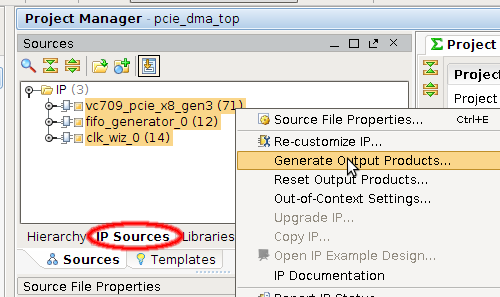
\includegraphics[width=0.75\textwidth]{pictures/generate_output_products.png}
\caption{Generate IP Cores output products}
\label{fig:generate_output_products}
\end{figure}
\subsection{Running synthesis and implementation}
When the project has been created, you can simply press the buttons to run synthesis and implementation of the design, but a tcl script has been created to run these steps automatically. Additionally the script will create the bitfile in the \textit{firmware/output} directory, as well as an .mcs file and an .ltx file, containing the ChipScope ILA probes. All those 3 files have a timestamp in their filename so any previous synthesis output will be maintained.
The script can simply be executed if the project is open. Please note that the script will fail if an already synthesized design is open.
\begin{lstlisting}[frame=single, language=tcl, caption=start synthesis / implementation]
cd /path/to/svn/checkout/firmware/scripts/pcie_dma_top/
source ./do_synt.tcl
\end{lstlisting}
\newpage


